\documentclass{article}
\usepackage{xcolor}
\usepackage{tikz}
\usetikzlibrary{scopes}
\usepackage{ifthen}
\usepackage[default]{gfsneohellenic}
\usepackage[LGR,T1]{fontenc}
\usetikzlibrary{shapes}
		
\begin{document}
	\pagestyle{empty}
	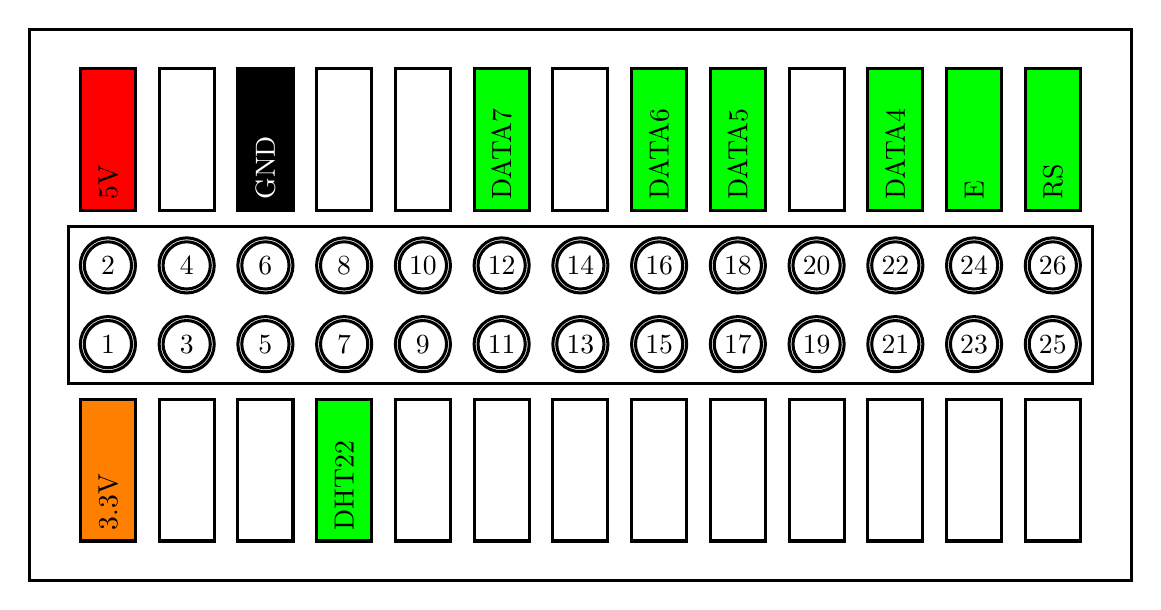
\begin{tikzpicture}[line width=1.1pt]
		\draw(-0.5,-2.5) rectangle (13.5, 4.5);
		\draw(0,0) rectangle (13,2);

		\foreach \x [
			evaluate = \x as \toppin using int(\x*2),
			evaluate = \x as \bottompin using int(\x*2-1)
		] in {1,...,13} {
			\ifthenelse{\x = 1}
				{\draw[fill=red] (\x-0.85,2.2) rectangle (\x-0.15,4);
			 	 \draw[fill=orange] (\x-0.85,-0.2) rectangle (\x-0.15,-2);}
				{\ifthenelse{\x = 3} % if 3
					{\draw[fill=black] (\x-0.85,2.2) rectangle (\x-0.15,4);
			 		 \draw (\x-0.85,-0.2) rectangle (\x-0.15,-2);}
					{\ifthenelse{\x = 4}
						{\draw (\x-0.85,2.2) rectangle (\x-0.15,4);
			 			 \draw[fill=green] (\x-0.85,-0.2) rectangle (\x-0.15,-2);}
						{\ifthenelse{\x = 6 \OR \x = 8 \OR \x = 9 \OR \x = 11 \OR \x = 12 \OR \x = 13}
							{\draw[fill=green] (\x-0.85,2.2) rectangle (\x-0.15,4);
							 \draw (\x-0.85,-0.2) rectangle (\x-0.15,-2);}
							{\draw (\x-0.85,2.2) rectangle (\x-0.15,4);
			 \draw (\x-0.85,-0.2) rectangle (\x-0.15,-2);
			 			}
					}
				}
			}
			\draw (\x-0.5,1.5) node {\toppin} circle (0.3) circle (0.35);
			\draw (\x-0.5,0.5) node {\bottompin} circle (0.3) circle (0.35);
			 
		}
			
		\newcommand{\pinlabel}[2]{%
			\ifthenelse{\isodd{#1}}%
				{\node[anchor=west,rotate=90] at (#1/2, -2) {#2}}%
				{\node[anchor=west,rotate=90] at (#1/2-0.5, 2.2) {\ifthenelse{#1 = 6}{\textcolor{white}{#2}}{#2}}}
		};
		
		\pinlabel{1}{3.3V};
		\pinlabel{2}{5V};
		\pinlabel{6}{GND};
		\pinlabel{7}{DHT22};
		\pinlabel{12}{DATA7};
		\pinlabel{16}{DATA6};
		\pinlabel{18}{DATA5};
		\pinlabel{22}{DATA4};
		\pinlabel{24}{E};
		\pinlabel{26}{RS};
	\end{tikzpicture}
\end{document}